\chapter{Конструкторская часть}

\section{Разработка алгоритма нахождения расстояния Левенштейна}

На рисунке \ref{img:lev} приведена схема итеративного алгоритма нахождения расстояния Левенштейна.
\begin{figure}[h]
	\centering
	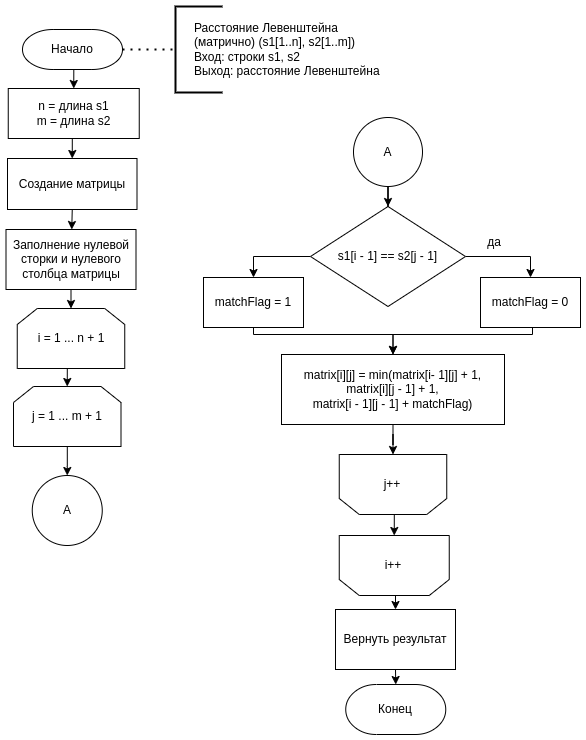
\includegraphics[width=140mm]{lev}
	\caption{Схема итеративного алгоритма нахождения расстояния Левенштейна}
	\label{img:lev}
\end{figure}

\section{Разработка алгоритмов нахождения расстояния Дамерау -- Левенштейна}

На рисунке \ref{img:damerau} приведена схема алгоритма нахождения расстояния Дамерау -- Левенштейна с заполнением матрицы.
\begin{figure}[h]
	\centering
	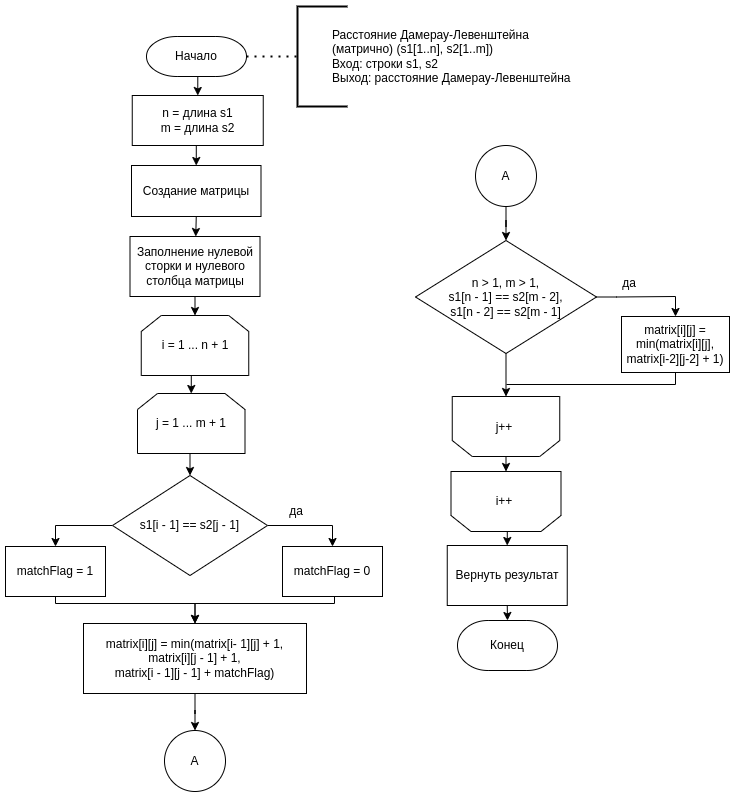
\includegraphics[width=170mm]{matrixDL}
	\caption{Схема итеративного алгоритма нахождения расстояния Дамерау -- Левенштейна}
	\label{img:damerau}
\end{figure}
\newpage
На рисунке \ref{img:recursive} приведена схема рекурсивного алгоритма нахождения расстояния Дамерау -- Левенштейна без кеширования. 
\begin{figure}[h]
	\centering
	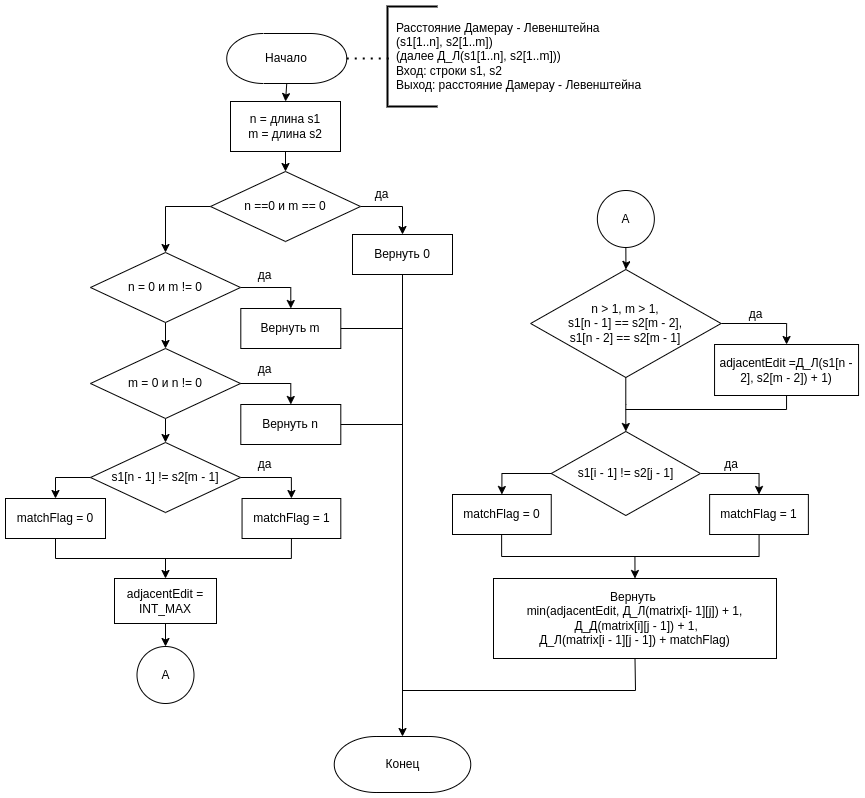
\includegraphics[width=175mm]{damerau}
	\caption{Схема рекурсивного алгоритма нахождения расстояния Дамерау -- Левенштейна без кеширования}
	\label{img:recursive}
\end{figure}
\newpage
На рисунке \ref{img:recursive_with_mem} приведена схема рекурсивного алгоритма нахождения расстояния Дамерау -- Левенштейна с кешированием.
\begin{figure}[h]
	\centering
	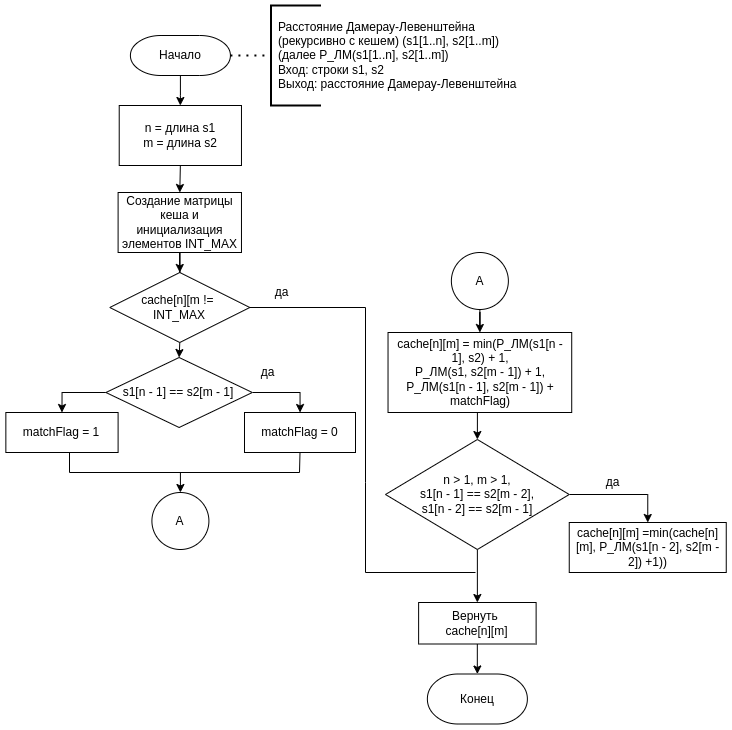
\includegraphics[width=160mm]{damerauCache}
	\caption{Схема рекурсивного алгоритма нахождения расстояния Дамерау -- Левенштейна с кешированием}
	\label{img:recursive_with_mem}
\end{figure}

